\documentclass[11pt]{article}

\usepackage{amsmath, mathtools, amsthm, graphicx, float, bm, csquotes}

\usepackage[backend=biber, style=authoryear, sorting=nyt, citestyle=authoryear, doi=false, isbn=false, url=false, eprint=false]{biblatex}

\addbibresource{references.bib}

\DeclareMathOperator{\di}{d\!}

\newcommand{\Unif}{\textit{Unif}[0,1]}

\newtheorem{proposition}{Proposition}

\begin{document}
\title{Diversity Incentives for Recruiters}
\author{Prasanna Parasurama}
\date{\today}
\maketitle

\begin{abstract}
    This paper concerns the effectiveness of diversity incentives for recruiters. I address whether incentives for recruiters to source diverse candidates are effective in increasing the diversity of the workforce. I first develop a theoretical model --  a 2-stage hiring game in which, recruiters are incentivized to shortlist the best candidates with an additional bonus for diverse candidates, and managers are incentivized to hire the best candidate from the shortlist with no diversity bonus -- and solve this model under the theory of rational choice under uncertainty. Second, I propose an experiment to test whether the empirics align with the theoretical predictions, and test whether behavioral concerns such as stereotyping countervail the intended effects of diversity incentives.
\end{abstract}

\section{Introduction}
Underrepresentation of women and minorities in the STEM labor force has far-reaching social and economic implications from untapped innovative capabilities to economic inequality. Organizations have attempted to address this issue in a multitude of ways: disclosing diversity reports, employing Diversity and Inclusion officers, and instituting policies to increase workforce diversity \parencite{shi_adoption_2018}. One such policy is an incentive scheme for recruiters to source and recruit diverse candidates. According to a Bloomberg article, Facebook implemented a point system in which recruiters get 1 point for every new hire and an additional point if the new hire is diverse \parencite{huet_facebooks_2017}. Recently, however, doubts have been raised about the effectiveness of this policy due to the misalignment of incentives between recruiters and engineers/managers, who ultimately make the hiring decision. Often, managers do not get extra incentives to hire diverse candidates, and often pass on them. The reporter in the article writes:
\begin{quote}
    The recruiters saw that many of their diversity candidates didn’t end up getting an offer. Two former recruiters blamed in part the engineering department’s candidate review process, a twice- or thrice-weekly meeting at which every engineering offer had to be approved \parencite{huet_facebooks_2017}.
\end{quote}

Similar phenomena have been pointed out by researchers as well. For example, in a recent research study that examines the effects of founder experience and gender on hire-ability, a recruiter interviewed by the authors is quoted:

\begin{quote}
    A technical recruiter at a search firm (Recruiter 16) who noted that “tons of companies come to us because all they want is diversity candidates” also stated that his clients are interviewing a lot of diversity candidates but not hiring them at the same rate \parencite{botelho_founder_2019}.

\end{quote}

This raises an important question of whether policies that incentivize recruiters to recruit diverse candidates are effective in ultimately increasing the diversity of the workforce, let alone not be counterproductive. While these policies are aimed to increase workforce diversity by putting more diverse candidates in front of managers, a countervailing effect is also possible: the existence of diversity bonuses may prejudice managers' beliefs about the quality of diverse candidates in a way that they are vastly (and incorrectly) underestimated, countervailing the intended effects of diversity policies. This possibility motivates the research questions of this paper: how effective are diversity incentive policies? Can diversity policies prejudice managers' beliefs about the quality of diverse candidates? To address these questions, I first develop a theoretical model that models the hiring process as a 2-stage game. I solve this model with assumptions of rational choice under uncertainty. I finally propose an experiment that tests the effectiveness of diversity incentive policies, and whether such policies prejudice managers' beliefs about the quality of diverse candidates.

\section{Literature}

There are two related strands of literature that are relevant in addressing the research questions at hand -- the economics literature on discrimination and the economics and social psychology literature on affirmative action programs. First, theories of discrimination in economics broadly fall into two categories: taste-based and statistical discrimination. In the labor context, theories of taste-based discrimination posit that an employer discriminates against individuals from certain groups because of the animus the employer has towards these groups -- that is, the employer derives disutility from hiring from certain groups \parencite{becker_economics_1971}. An alternative, but much more widely studied in economics, is the theory of statistical discrimination, wherein an employer who observes a noisy signal of applicants' productivity resorts to group-level averages and variances as proxies, leading to discrimination \parencite{arrow_theory_1973,phelps_statistical_1972,aigner_statistical_1977}. Unlike taste-based models, statistical discrimination assumes no animus on the part of the employer, but is a consequence of rational action. For example, given two applicants from two groups with similar, but noisy signals of productivity, the employer will hire the one from the group with higher average productivity. Similarly, a risk-averse employer will hire the one from the group with lower variance in productivity \parencite{aigner_statistical_1977}.

Dozens of studies have documented statistical and taste-based discrimination in labor market settings (See \cite{bertrand_chapter_2017,anderson_discrimination_2005,guryan_tastebased_2013} for a review). Some of these studies show how discrimination can arise even when populations are identical. Of particular relevance is a study by Davis, in which the author argues that if employers make inferences about group productivity from the maximum observation of productivity in the group, rather than average observation (for example, employers may remember the best candidate they hired more rather than they remember the average candidate), then the smaller group may be perceived as inferior -- since, the expected value of the maximum value is directly related to the number of observations in a group \parencite{davis_maximal_1987}. This nuanced distinction of discrimination based on incorrect beliefs has received attention in recent years. \citeauthor{bohren_inaccurate_2019}, for example, have articulated this distinction and called for a third type of discrimination -- inaccurate statistical discrimination -- for cases in which employers statistically discriminate based on their beliefs, but the beliefs themselves are inaccurate \parencite{bohren_inaccurate_2019}. This is precisely the countervailing effect pointed out at the beginning of this paper -- the presence of diversity incentives may dispose managers to vastly underestimate the productivity of diverse candidates -- more so than what is statistically warranted. The literature on affirmative action programs gives some insights into the mechanism behind this.

While studies have documented positive aspects of affirmative action policies (AAPs) -- such as increased effort levels, increased overall output, increased diversity \parencite{schotter_asymmetric_1992,balafoutas_affirmative_2012,niederle_how_2012}, a number of studies have also pointed out its negative impacts. It is widely documented that in the presence of AAPs, majority groups stigmatize AAP hires and view them as less competent \parencite{leslie_stigma_2013,heilman_affirmative_1997,petters_negative_2020}. These negative views are extended to other members of affirmed groups even if they are not hired under AAPs. Furthermore, AAP hires and minorities may view themselves as less competent due to stereotype threat, which in turn affects performance, creating a vicious cycle \parencite{leslie_stigma_2013}. While these studies give insights into mechanisms and outcomes of AAPs in general, a fundamental limitation (at least with respect to the diversity incentive policy described in this paper) is that these policies are exogenously imposed. To my knowledge, none of the studies sufficiently capture the incentive misalignment between the recruiter and the manager, further motivating this study.


\section{Theoretical Model and Predictions}

\subsection{Model}

To formalize the diversity incentive policy described above, I develop a simple model that models the hiring process as a 2-stage game.
In the first stage, the recruiter receives applications from $n_a$ applicants, of which $n_m$ are male and $n_f$ are female. Each candidate has productivity $q$, which is a random variable drawn from a distribution with cumulative distribution function $F_q(\cdot)$ and density function $f_q(\cdot)$. Even though the recruiter doesn't observe the true productivity $q$, he\footnote{I will use the pronouns ``he'' and ``she'' to refer to the recruiter and the hiring manager respectively.} observes a noisy signal of productivity, $\hat{q_r}$, which is correlated with the true productivity -- this is akin to recruiters inferring applicants' productivity from resumes, for example.
The recruiter's task is to shortlist $n_s$ candidates to send to the manager. He receives a payout that is proportional to the productivity of the candidate hired by the manager ($c_rq$), and receives an additional diversity bonus, if the hired candidate is female ($c_rq + bq$). Formally, the recruiter's utility function is:

\[  U_r =
    \begin{cases}
        c_rq     & \textit{if male is hired}             \\
        (b+c_r)q & \textit{if female is hired}, b \geq 0
    \end{cases}
\]

In the second stage of the game, the hiring manager receives $n_s$ shortlisted candidates from the recruiter. Like the recruiter, the manager also has her own assessment of the candidate's productivity $\hat{q}_h$, and her task is to hire $n_h$ candidates. The manager receives a payout that is proportional to the applicant's true productivity $q$, but receives no additional bonus for hiring a female candidate. The manager's utility function is thus:

$$U_h = c_hq$$

\subsection{Rational Choice under Uncertainty}

In this section, I simplify the above model by fixing some parameters, and solve the simplified model under expected utility theory (rational choice under uncertainty). This will serve as a baseline comparison for experimental results.

Assume that the true productivity of both male and female candidates are identically distributed under $\textit{Unif}[0,1]$, and that this is common knowledge.
The recruiter's task is to send 2 candidates to the manager. However, for mathematical tractability, instead of shortlisting 2 candidates in the same round, the recruiter shortlists 2 candidates in 2 sub-rounds -- that is, he shortlists 1 candidate in the first round and shortlists another in the subsequent round. The manager receives 2 candidates in total (from 2 sub-rounds), and her task is to hire 1 candidate.

Without loss of generality, further assume that the recruiter's and manager's commissions are both 1, $c_r=c_h=1$. For brevity, redefine $b$ so that $b \geq 1$. Instead of writing $U_{r,f} = (1+b)q, b \geq 0$  define $U_{r,f} = bq, b \geq 1$.

\begin{align*}
     & q \sim \textit{Unif}[0,1] \\
     & U_r =
    \begin{cases}
        q  & \textit{if male is hired}             \\
        bq & \textit{if female is hired}, b \geq 1
    \end{cases}    \\
     & U_h = q
\end{align*}

In each round, given there are $n_m$ male and $n_f$ female candidates in a set of applicants $\bm{a}=\{m_1, m_2, f_3...f_{n_m+n_f}\}$, with corresponding productivities $\{q_1...q_{n_m+n_f}\}$, and recruiter's utilities $\{U_1...U_{n_m+n_f}\}$, the recruiter will shortlist a candidate that will maximize his expected utility. Since the manager has to hire a candidate, the recruiter's optimal strategy is to shortlist the candidate with the highest utility in each round. Note that this utility is a function of the candidate's productivity, gender of the candidate, as well as the diversity bonus.
$$S \equiv \max_{\bm{a}} U_r(q, b, \textit{gender})$$

Likewise, given a set of shortlisted candidates $\bm{s}=\{m_1...f_{n_s}\}$, the manager will hire a candidate that maximizes her own expected utility, which is only a function of the candidate's productivity.

$$\max_{\bm{s}} U_h(q)$$

\begin{table}
    \caption{Table of Notations}
    \begin{center}

        \begin{tabular}{ l l}
            \hline
            Symbol       & Definition                                             \\
            \hline
            $F_X(\cdot)$ & Cumulative distribution function of $X$                \\
            $f_X(\cdot)$ & Probability density function of $X$                    \\
            $m$          & Male                                                   \\
            $f$          & Female                                                 \\
            $\bm{a}$     & Set of applicants                                      \\
            $\bm{s}$     & Set of shortlisted candidates                          \\
            $q$          & Candidate's true productivity                          \\
            $\hat{q}_r$  & Recruiter's belief about candidate's productivity      \\
            $\hat{q}_h$  & Hiring manager's belief about candidate's productivity \\
            $b$          & Recruiter's diversity bonus                            \\
            $U_r$        & Recruiter's utility                                    \\
            $S$          & Max of recruiter's utility from a list of applicants   \\
            $U_h$        & Hiring manager's utility                               \\
        \end{tabular}
    \end{center}


\end{table}


\begin{proposition}
    The probability that a male (female) is shortlisted decreases (increases) with diversity bonus $b$.
\end{proposition}

\begin{proof}
    Given the productivies of male and female candidates are uniformly distributed, the recruiter's utility from male and female candidates are also uniformly distributed:
    \begin{align*}
         & U_{r,m} \sim \Unif              \\
         & U_{r,f} \sim \textit{Unif}[0,b]
    \end{align*}

    Let $S_m$ and $S_f$ be the maximum utility to be gained from male and female candidate respectively:
    $S_m=Max(U_{r_m})$ and $S_f=Max(U_{r_f})$. Note that $S_m$ and $S_f$ are $n^{th}$ order statistic of a uniform distribution, with the following CDFs:

    \begin{align*}
         & F_{S_m}(x) =
        \begin{cases}
            x^{n_m} & 0 < x < 1 \\
            1       & x \geq 1  \\
            0       & otherwise
        \end{cases}
        \\
         & F_{S_f}(x) =
        \begin{cases}
            \frac{x}{1+b}^{n_f} & 0 < x < b \\
            1                   & x \geq b  \\
            0                   & otherwise
        \end{cases}
    \end{align*}


    A male candidate is shortlisted when the maximum utility gained from a male candidate exceeds the maximum utility gained from a female candidate: $S_m=Max(U_{r_m}) > S_f=Max(U_{r_f})$. Then, the probability that a male is shortlisted is:
    \begin{align*}
        Pr(S_m > S_f) & = Pr(S_f = x) Pr(S_m > x)                        \\
                      & = \int_{0}^{b+1} f_{S_m}(x) (1-F_{S_f}(x)) \di x \\
                      & = \frac{(b+1)^{-n_f} n_m}{n_f+n_m}
    \end{align*}

    Since $n_m, n_f >0$, the above expression is decreasing with bonus $b$.

\end{proof}

\begin{proposition}\label{prop_male_exp_qual}
    The expected productivity of a shortlisted male candidate is independent of diversity bonus $b$.
\end{proposition}
\begin{proof}
    Consider the conditional density function of the recruiter's utility from a male candidate that is shortlisted,  $f_{S_m|S_m>S_y}$. This conditional density function can be written as:

    \begin{align*}
        f_{S_m|S_m>S_f}(x) & = \frac{f_{S_m}(x)F_{S_f}(x) }{Pr(S_m > S_f)}     \\
                           & = \frac{(n_f+n_m)(x^{n_f+n_m-1})}{n_mBeta[n_m,1]}
    \end{align*}

    Expected utility from a shortlisted male candidate is then:

    \begin{align*}
        E[S_m|S_m > S_y] & = \int_0^1{xf_{S_m|S_m>S_y}(x) \di x} \\
                         & = \frac{n_m + n_f}{1+n_f+n_m}
    \end{align*}

    Since $U_r = q$ for male candidates:

    $$E[q_m|S_m > S_y] = \frac{n_m + n_f}{1+n_f+n_m}$$

    which is independent of diversity bouns $b$.
\end{proof}


\begin{proposition}\label{prop_female_exp_qual}
    The expected productivity of a shortlisted female candidate decreases with diversity bonus $b$.
\end{proposition}
\begin{proof}
    Following the above proof, the conditional density function of the recruiter's utility of a shortlisted female candidate is

    \begin{align*}
        f_{S_f|S_f>S_m}(x) & = \frac{f_{S_f}(x)F_{S_m}(x) }{Pr(S_f > S_m)} \\
                           & = \begin{cases}
            \frac{n_f(n_f+n_m)x^{(n_f-1)}x^{n_m}}{-n_m+b^{n_f}(n_f+n_m)} & 0 \leq x < 1    \\
            \frac{n_f(n_f+n_m)x^{(n_f-1)}}{-n_m+b^{n_f}(n_f+n_m)}        & 1 \leq x \leq b \\
        \end{cases}
    \end{align*}

    The expectation of the recruiter's utility from a shortlisted female candidate is:

    \begin{align*}
        E[S_f|S_f > S_m] & = \int_0^1{x \frac{ n_f(n_f+n_m)x^{(n_f-1)}x^{n_m}}{-n_m+b^{n_f}(n_f+n_m)} \di x}                 \\
                         & + \int_1^b{x \frac{n_f(n_f+n_m)x^{(n_f-1)}}{-n_m+b^{n_f}(n_f+n_m)} \di x}                         \\
                         & = \frac{n_f(n_f+n_m)(-n_m+b^{(1+n_f)} (1+n_f+n_m))}{(1+n_f) (1+n_f+n_m) (-n_m+b^{n_f} (n_f+n_m))}
    \end{align*}

    Since the recruiter's utility is $U_r = bq \implies q = \frac{U_r}{b}$ for female candidates,
    \begin{align*}
        E[q_f|S_f > S_m] & = \frac{1}{b} \frac{n_f(n_f+n_m)(-n_m+b^{(1+n_f)} (1+n_f+n_m))} {(1+n_f) (1+n_f+n_m) (-n_m+b^{n_f} (n_f+n_m))}
    \end{align*}

    Taking the derivative of the above expression with respect to $b$:
    \begin{align*}
         & \frac{\di E[q_f|S_f > S_m]} {\di b}  =                                                                                                                             \\
         & - \frac{[n_f n_m (n_f+n_m)] [\left(-(n_f+1) b^{n_f} (n_f+n_m)+n_f b^{n_f+1} (n_f+n_m+1)+n_m\right)]}{b^2 (n_f+1) (n_f+n_m+1) \left(n_m-b^{n_f} (n_f+n_m)\right)^2}
    \end{align*}

    Note that the two terms in the numerator and the term on the denominator are positive for $n_m, n_f, b \geq 1$, making the whole term negative.

\end{proof}

\begin{proposition}
    Given a shortlist containing 1 male and 1 female candidate $\bm{s} = \{m,f\}$, the probability that a male (female) is hired increases (decreases) with diversity bonus $b$.
\end{proposition}

\begin{proof}
    The intuition for this proposition is as follows: bonus $b$ changes the productivity distribution of a shortlisted female, which in turn affects the conditional probability that a male is hired. As bonus $b$ increases, the expected productivity of a shortlisted female decreases (Proposition \ref{prop_female_exp_qual}), however the expected productivity of a shortlisted male remains the same (Proposition \ref{prop_male_exp_qual}). As a result, the conditional probability that a male is hired increases.

    Formally, consider the conditional probability that a male is hired given a shortlist $\bm{s}=\{m,f\}$ (i.e. one male, one female), and define it as $Pr(n_{h_m}=1|\bm{s}=\{m,f\})$. This is the probability that the productivity of the shortlisted male exceeds the productivity of the shortlisted female:
    \begin{align*}
        Pr(\textit{Male is hired}|\bm{s}=\{m,f\}) & \equiv Pr(n_{h_m}=1|\bm{s}=\{m,f\})     \\
                                                  & = Pr([q_m|S_m > S_f] > [q_f|S_f > S_m])
    \end{align*}

    where $q_m|S_m > S_f$ and $q_f|S_f > S_m$ are the productivities of shortlisted male and female respectively. From Proposition \ref{prop_male_exp_qual}, we know the distribution of the recruiter's utility from a shortlisted male. Because the recruiter's utility equals the productivity for male candidates ($U_{r,m} = q$), the productivity of shortlisted male follows the same distribution as the recruiter's utility.

    \begin{align*}
        f_{q_m|S_m > S_y} = f_{S_m|S_m > S_y} = \frac{(n_f+n_m)(x^{n_f+n_m-1})}{n_mBeta[n_m,1]}
    \end{align*}

    For female candidates, we know the distribution of the recruiter's utility from a shortlisted female candidate. Using the change of variable technique with respect to the function $g: U_{r,f} = bq$, we can get the productivity distribution of a shortlisted female.

    \begin{align*}
        f_{q_f|S_f > S_m}(x) & = f_{S_f|S_f > S_m} (g^{-1}(x)) \lvert \frac{\di}{\di x} (g^{-1}(x)) \rvert \\
                             & = \frac{n_f (n_f+n_m) x^{n_f-1} \left(
            \begin{array}{cc}
                     &
                    \begin{array}{cc}
                        x^{n_m} & 0<x<1 \\
                    \end{array}
                    \\
                \end{array}
            \right)}{b^{n_f} (n_f+n_m)-n_m}
    \end{align*}

    Using these two distributions:

    \begin{align*}
         & Pr(n_{h_m=1}|bm{s}=\{m,f\})                                                                                                                             \\
         & = Pr([q_m|S_m > S_f] > [q_f|S_f > S_m])                                                                                                                 \\
         & = \int_{0}^{b+1} f_{q_m|S_m > S_f}(x) (1-F_{q_f|S_f > S_m}(x)) \di x                                                                                    \\
         & = \frac{b^{-n_f-n_m} \left(-2 n_m (2 n_f+n_m) b^{n_f+n_m}+2 (n_f+n_m)^2 b^{2 n_f+n_m}+n_f n_m\right)}{2 (2 n_f+n_m) \left(b^{n_f} (n_f+n_m)-n_m\right)}
    \end{align*}

    Taking the derivative of the above expression w.r.t $b$:
    \begin{align*}
         & \frac{\di}{\di b} Pr(n_{h_m=1}|bm{s}=\{m,f\})                                                                                                             \\
         & = \frac{n_f n_m (n_f+n_m) b^{-n_f-n_m-1} \left(b^{n_f} (-(2 n_f+n_m))+2 n_f b^{2 n_f+n_m}+n_m\right)}{2 (2 n_f+n_m) \left(n_m-b^{n_f} (n_f+n_m)\right)^2}
    \end{align*}

    which is positive for $b, n_m, n_f \geq 1$.

\end{proof}


\begin{proposition}
    The overall probability that a male (female) is hired decreases (increases) with diversity bonus $b$.
\end{proposition}

\begin{proof}
    The overall probability that a male is hired depends on both the probability that a male is shortlisted and the probability that a male is hired given a shortlist.

    Recall that $Pr(n_{h,m}=1|\bm{s})$ is the conditional probability that a male is hired given shortlist $\bm{s}$. Further define $Pr(n_{h,m}=1)$ as the overall probability that a male is hired, and $n_{s,m}$ as the number of shortlisted males.

    \begin{align*}
         & Pr(\textit{Male is Hired}) \equiv Pr(n_{h,m}=1)                               \\
         & = \sum\nolimits_{n_{s,m} \in \{0,1,2\}} Pr(n_{h,m}=1|\bm{s}) Pr(n_{s,m})      \\
         & = Pr(n_{s,m} = 0)Pr(n_{h,m}=1|\{f,f\}) + Pr(n_{s,m} = 1)Pr(n_{h,m}=1|\{m,f\}) \\
         & \qquad + Pr(n_{s,m} = 1)Pr(n_{h,m}=2|\{m,m\})
    \end{align*}

    Note that $Pr(n_{s,m})$ has a binomial distribution with parameter $p=Pr(\text{Male is shortlisted})=\frac{(b+1)^{-n_f} n_m}{n_f+n_m}$ and $n=2$. Substituting this in:

    \begin{align*}
        Pr(n_{h,m}=1) & = \binom{2}{0}p^0(1-p)^2 Pr(n_{h,m}=1|\bm{s}) +  \binom{2}{1}p(1-p) Pr(n_{h,m}=1|\bm{s})                                           \\
                      & \qquad + \binom{2}{2}p^2(1-p)^0 Pr(n_{h,m}=1|\bm{s})                                                                               \\
                      & =  0 + \binom{2}{1}p(1-p) Pr(n_{h,m}=1|\bm{s}) + \binom{2}{2}p^2(1-p)^0                                                            \\
                      & = \frac{n_m b^{-3 n_f-n_m} \left(-n_m (2 n_f+n_m) b^{n_f+n_m}+2 (n_f+n_m)^2 b^{2 n_f+n_m}+n_f n_m\right)}{(n_f+n_m)^2 (2 n_f+n_m)}
    \end{align*}

    Taking the derivative of the above expression with respect to $b$:

    \begin{align*}
         & \frac{\di}{\di b} Pr(n_{h,m}=1) =                                                                                                         \\
         & -\frac{[n_f n_m b^{-3 n_f-n_m-1}] [-2 n_m (2 n_f+n_m) b^{n_f+n_m}+2 (n_f+n_m)^2 b^{2 n_f+n_m}+n_m (3 n_f+n_m)])}{(n_f+n_m)^2 (2 n_f+n_m)}
    \end{align*}

    Because $n_m, n_f, b \geq 1$, the first term on the numerator and the denominator are always positive. Part of the second term can be written as:
    \begin{align*}
        -2 n_m (2 n_f+n_m) b^{n_f+n_m}+2 (n_f+n_m)^2 b^{2 n_f+n_m} & = \\
        2b^{2n_f+n_m} + 4b^{2n_f+n_m} n_f n_m + 2b^{2n_fn_m} m^2 - 4b^{n_fn_m}n_fn_m - 2b^{n_f+n_m}m^2
    \end{align*}

    Since $4b^{2n_f+n_m} n_f n_m > 4b^{n_fn_m}n_fn_m$ and $2b^{2n_fn_m} m^2 > 2b^{n_f+n_m}m^2$ for $n_f,n_m,b \geq 1$, the second term is also positive. This makes the derivative negative.
\end{proof}

\subsection{Inaccurate Beliefs}

A fundamental assumption in rational choice theory is that the manager's (and recruiter's) beliefs about the productivity of shortlisted candidates are independent of diversity bonus $b$ -- that is $\hat{q}_r$ and $\hat{q}_m$ are independent of $b$, controlling for true productivity $q$. Of course, as discussed before, psychological biases and stereotyping brings this assumption into question. The presence of diversity bonus may prejudice managers' beliefs about the productivity of diverse candidates leading them to vastly underestimate their productivity.  Part of the experiment proposed in the following section tests whether this is the case.

\section{Experimental Setup}

The experiments are aimed to closely mirror the theoretical model described in section 2. Participants are recruited and separated into two groups -- recruiters and hiring managers. Each recruiter is matched with a hiring manager, and they play a hiring game in which they hire a candidate together. They play 10 rounds total (10 total hires) before the participants are rematched.  Note that this is a between-subject design -- once a participant is assigned to a treatment cell, it will not change throughout the experiment. Managers and recruiters are informed of their own payment structure, as well as their counterparty's payment structure. In addition, both the managers and recruiters receive the full set of instructions, so everything below is common knowledge.
\\

In each round, each recruiter receives 4 resumes (3 male, 1 female candidate)\footnotemark, which contains the candidate's name, GPA, Degree, Field of Study, and Years of Experience. The gender of the candidate is made salient by the name. Recruiters are asked to assess each candidate's productivity and shortlist 1 or 2 candidates for a fictional software engineering job. They are further informed that the true productivity $q$ of the candidate is composed of two components: first, a deterministic productivity score $q'$ that depends on the candidate's credentials (GPA, Degree, Field of Study, Yrs of Experience). They are shown a schema for how productivity score $q'$ is related to credentials as well as some examples. In general, the higher the GPA, Yrs of Experience, and Degree, and more technical the field of study, the higher the score. Second, there is a random error term $\delta$, that is added to the score. This implies that in some cases, even if a candidate has stellar credentials, their true productivity may be less than stellar; but in general, better credentials mean higher productivity. Recruiters are informed that the distribution of productivity among male and female candidates is the same in the initial candidate pool -- that is, on average, a male candidate has the same productivity as a female candidate.


$$q = 0.7q' + 0.3\delta$$
$$q' = f(\textit{GPA, Degree, Field of Study, Yrs Exp})$$


\footnotetext{This roughly reflects the actual gender proportion in software engineering jobs.}

\begin{figure} % not "pt"
    \centering
    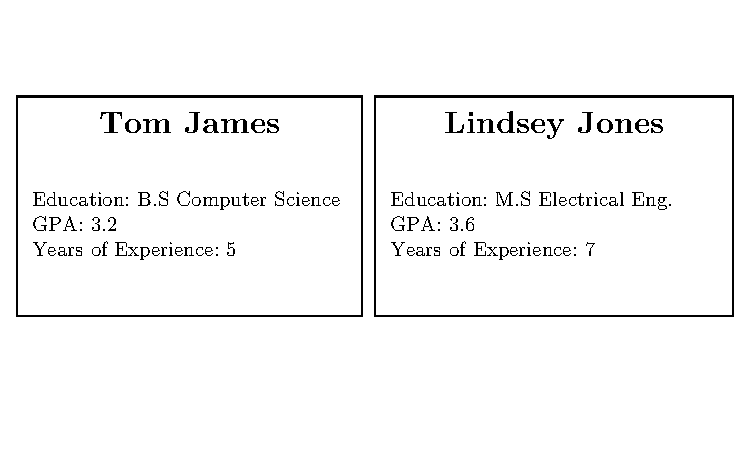
\includegraphics[width=\textwidth, keepaspectratio]{illus/resumes.pdf}
    \caption{Illustration of Resumes}
    \label{sample_resumes}
\end{figure}

Once a recruiter shortlists 2 candidates, the manager receives the resumes of the shortlisted candidates. The manager is asked to assess each candidate's productivity and hire one candidate. Once the manager hires a candidate, the true productivity of the hired candidate is revealed to both the recruiter and the manager, and both receive a payout based on the candidate's true productivity.

\subsubsection*{Eliciting Beliefs about Candidate Productivity}

In each round, for each candidate, participants are also asked to record their beliefs of the candidate's productivity $\hat{q}_r$ and $\hat{q}_h$. To incentivize and elicit true beliefs about candidate productivity, some rounds are randomly chosen, and participants are awarded an additional payout that is related to the distance between belief and the true productivity: $1-|q - \hat{q}|$.

\subsubsection*{An Alternative Setup}

An alternative setup that abstracts away from the hiring context (and predisposed beliefs about the gendered nature of software engineering jobs) is to have ``recruiters'' and ``managers'' assess the angle of different colored vertices. In this setup, the angle corresponds to the productivity score of the candidate, and the colors correspond to the gender. This greatly reduces the complexity of the task, but comes at the cost of external validity.

\begin{figure}[H] % not "pt"
    \centering
    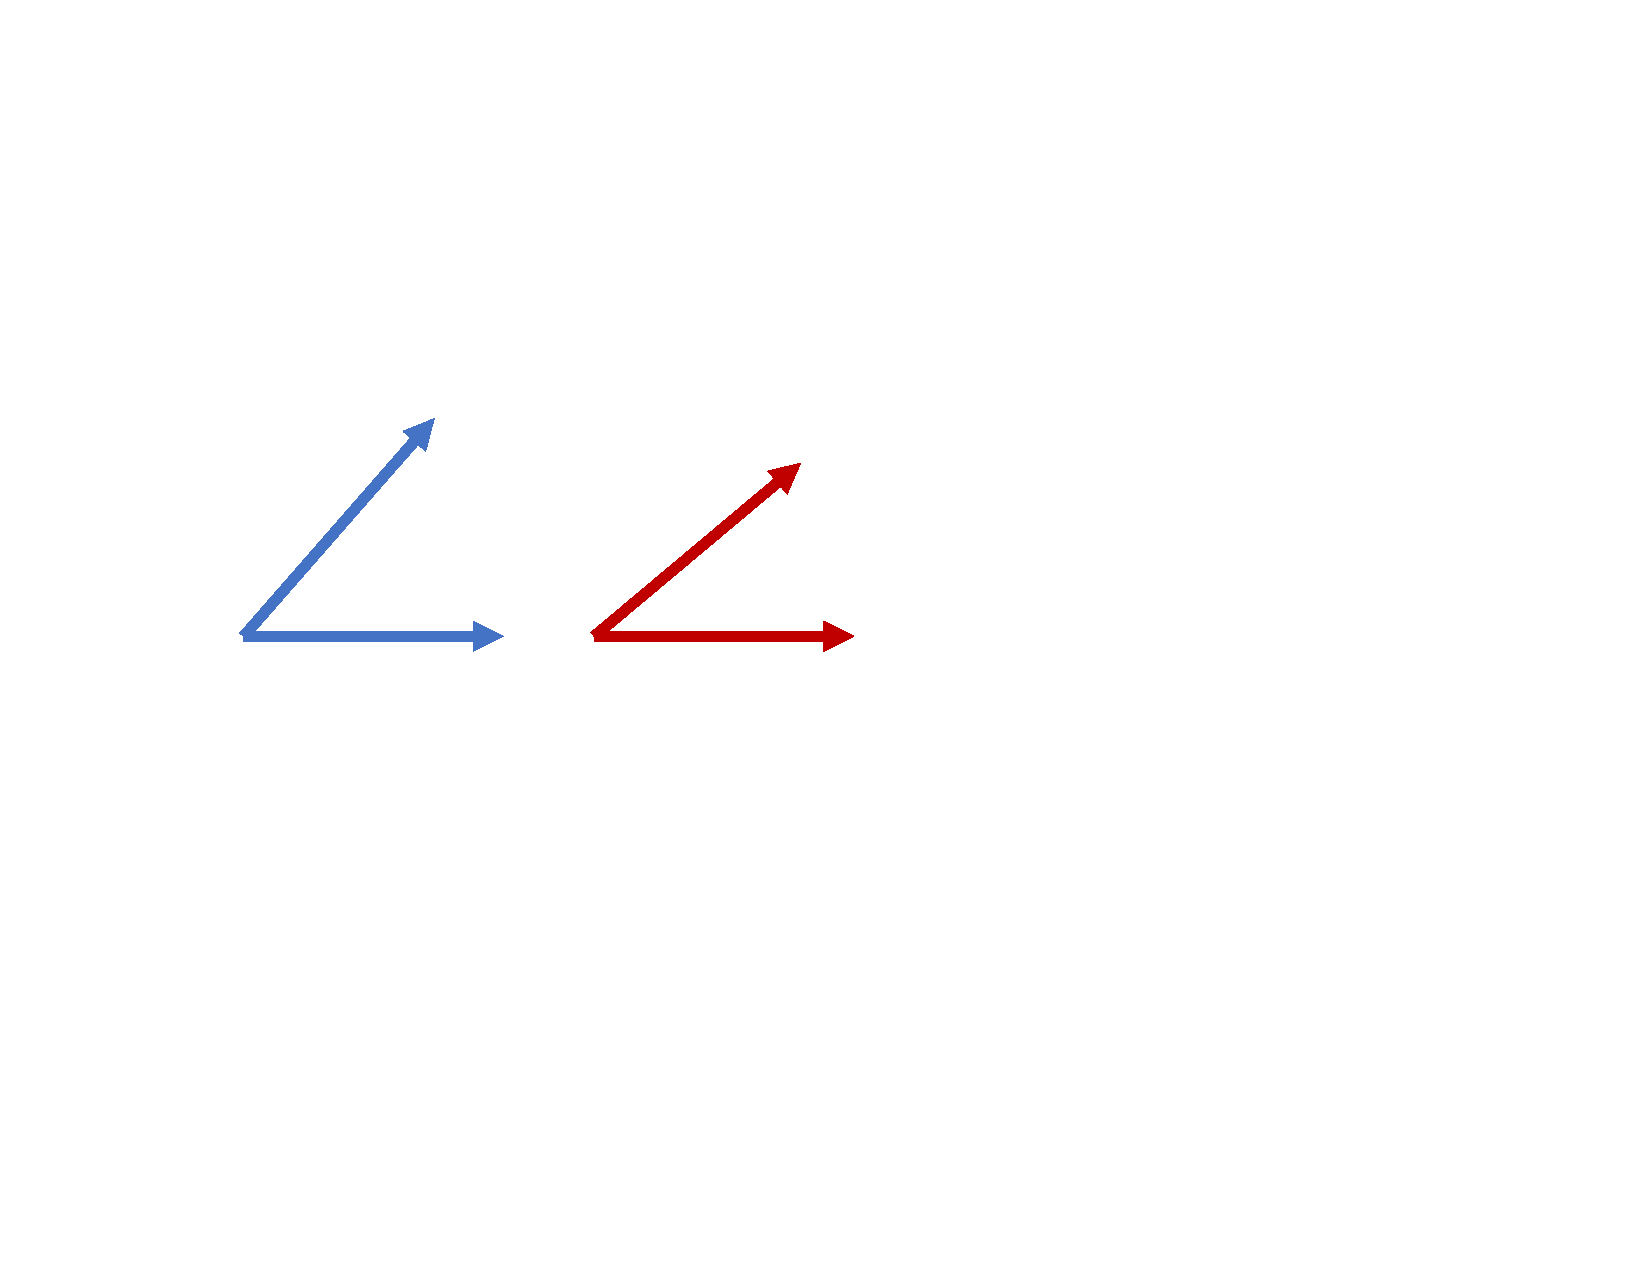
\includegraphics[width=\textwidth, keepaspectratio]{illus/angles.pdf}
    \caption{Illustration of Angles}
    \label{sample_angles}
\end{figure}

\subsection{Experimental Variables and Parameters}

The main variable of interest is diversity bonus, which will be varied at the following levels: no diversity bonus $b=1$, which serves as the control; 50\% diversity bonus $b=1.5$ (Treatment 1), and 100\% diversity bonus $b=1$ (Treatment 2). With $b=1.5, n_m=3, n_f=1$, there is a 50\% chance that a male candidate is shortlisted. This will ensure that the manager sees roughly an equal number of male and female candidates.

In the theoretical model, recruiters are assumed to shortlist 2 candidates in 2 separate sub-rounds. Although this assumption makes the model tractable, it may be too contrived. To address this, an alternate setup is also tested, in which recruiters shortlist 2 candidates in the same round. This is to check whether the empirical results deviate between the two setups.

If resources permit, the proportion of male to female candidates in the initial pool can also be varied.

\begin{center}
    \begin{tabular}{ l l}
        \hline
        Variable                                       & Values    \\
        \hline
        Diversity bonus $b$                            & $1,1.5,2$ \\
        Number of sub-rounds to shortlist 2 candidates & 1,2       \\
        Number of Male/Female candidates               & 3/1,2/2
    \end{tabular}
\end{center}


\subsubsection*{Power Analysis}
Assuming a standard deviation of 0.1, to detect a 10\% effect size of probability that a male is hired with 80\% power at $\alpha=0.05$, we require a sample size of 120 participants in each treatment cell.

\subsection{Data Generating Process}

As mentioned earlier, the candidate's true productivity $q$ is composed of 2 components: a deterministic productivity score $q'$, which is a function of the candidate's credentials, and a random disturbance term $\delta$. $q'$ has a uniform distribution $q' \sim \Unif$. Because the true productivity $q$ also needs to be bounded between 0 and 1, a logit and inverse-logit transform is performed on gaussian noise. This ensures that $q$ is roughly uniformly distributed and bounded between 0 and 1.

$$q_i        = 0.7q'_i + 0.3\delta_i$$
$$q_i'= f(\textit{GPA}_i, \textit{Degree}_i, \textit{FieldofStudy}_i, \textit{YrsExp}_i)$$
$$\delta_i = \frac{1}{1+ exp(-\mathcal{N}(q'_i, 1))}$$
$$q \sim \Unif$$

\subsection{Specification and Estimation}

The first set of analyses compares estimates of (1) Probability that a male is shortlisted, (2) Expected productivity of shortlisted males, (3) Expected productivity of shortlisted females, and (4) Probability that a male is hired, with their theoretical predictions. This involves a simple difference-in-means estimation.

Next, to test whether the presence of diversity bonus prejudices manager's beliefs about the productivity of diverse candidates, the following regression equation is estimated for each gender separately. Under rational choice, we expect $\beta_2$ and $\beta_3$ to be 0.
$$\hat{q}_{h,i} = \beta_0 + \beta_1q_i + \beta_2 b + \beta_3 q_i b + \epsilon_i$$

\subsection{Extensions}

If resources permit, an interesting extension to the experiment is to introduce competition among recruiters. Instead of each recruiter sending 2 candidates to the manager, in the presence of competition, each recruiter sends 1 candidate to the manager. In this setup, recruiters are more likely to be strategic.

\printbibliography

\newpage
\section*{Appendix}

\subsection*{A: Theoretical Predictions}

The following plots show the predicted probability of being shortlisted and hired, and the expected productivity of candidates as a function of diversity bonus $b$, given $n_m=3, n_f=1$

\begin{figure}[H] % not "pt"
    \centering
    \caption{Probability of being shorlisted}
    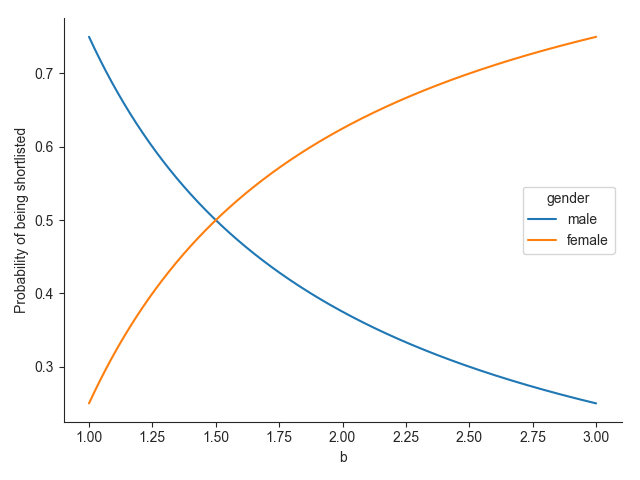
\includegraphics[width=\textwidth, keepaspectratio]{plots/prob_shortlist.png}

\end{figure}

\begin{figure}[H] % not "pt"
    \centering
    \caption{Conditional probability of being hired given shortlist $\bm{s} = \{m,f\}$}
    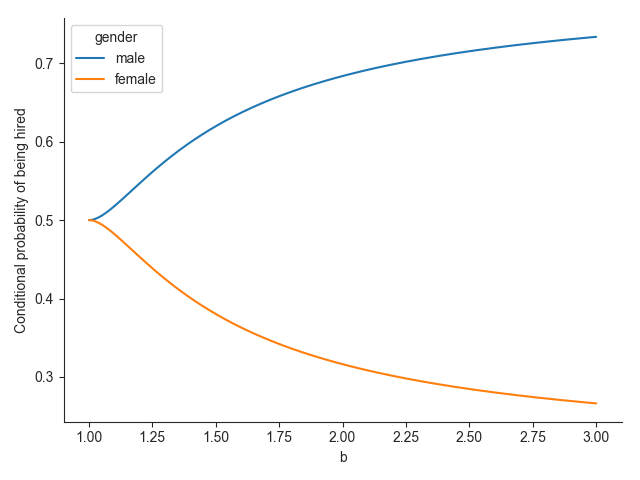
\includegraphics[width=\textwidth, keepaspectratio]{plots/conditional_prob_hire.png}
\end{figure}


\begin{figure}[H] % not "pt"
    \centering
    \caption{Overall probability of being hired}
    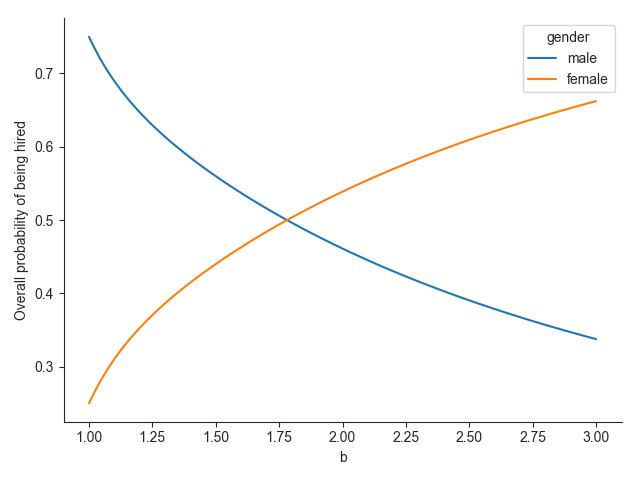
\includegraphics[width=\textwidth, keepaspectratio]{plots/overall_prob_hire.png}
\end{figure}

\begin{figure}[H] % not "pt"
    \centering
    \caption{Expected productivity of a shortlisted candidate}
    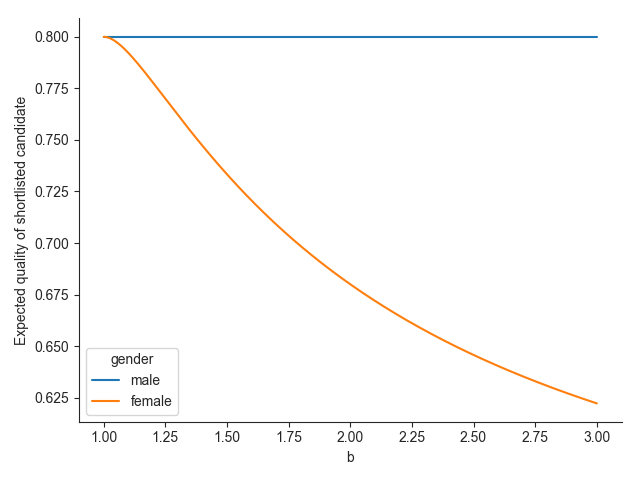
\includegraphics[width=\textwidth, keepaspectratio]{plots/expected_quality_shortlist.png}
\end{figure}




\end{document}

